\documentclass[a4paper, oneside]{memoir}% Document class
\usepackage[a4paper]{geometry}			% Margins
\usepackage{lmodern}
\usepackage{graphicx}
\usepackage{float}
\usepackage{listings}
\usepackage[small,compact]{titlesec}	% No 'chapter' in chapter headings.
\graphicspath{{Media/}}					% Directory that holds images.

\titleformat{\chapter}[hang]
{\normalfont\Large\bfseries}{\thechapter}{1em}{\Large}
\titlespacing{\chapter}{0pt}{*0}{*1}

\titleformat{\chapter}{\Huge\bfseries}{\thechapter}{1em}{}
\titleformat{\section}{\LARGE\bfseries}{\thesection}{1em}{}
\titleformat{\subsection}{\Large\bfseries}{\thesubsection}{1em}{}
\titleformat{\subsubsection}{\normalsize\bfseries}{\thesubsubsection}{1em}{}


\author{
  Lasse Vang Gravesen\\
  \texttt{lgrave11@student.aau.dk}
  \and
  Dennis Jakobsen\\
  \texttt{djakob11@student.aau.dk}
  \and
  Erik Sidelmann Jensen\\
  \texttt{ejens11@student.aau.dk}
}

\title{DIS Miniproject}
\date{}

\begin{document}
	\clearpage\maketitle
	\thispagestyle{empty}
	%\tableofcontents
	
	\chapter{DIS Miniproject}
	\section{Task B}
	\begin{itemize}
	\item Sales
	\item Payments
	\item Members
	\item Location
	\end{itemize}
	
	We pick the 'Sales' business process, because it is the most interesting. Granularity with regards to time sales it is important to have a lot of detail, so we choose the specific date and time. ?? Is it reasonable for a paying customer???  
	
	Examples of questions:
	\begin{itemize}
	\item How much is bought at some point during some day?
	\item How does the amount sold change over time?
	\item Which days are the most busy?
	\item When is it best to restock, given low activity?
	\item How much revenue is gained each day, week, month, year?
	\item Which products have changed the most in price from year to year?
	\item Which department or member have spent the most?
	\end{itemize}


	\section{Task C}
	The business process proposed to be modelled in the data warehouse is the 'Sales' business process. With regards to dimensions we pick out product, time, date, and member because those are the most interesting dimensions. Our granularity with regards to time goes down to minutes across two different dimensions to reduce the amount of rows, with regard to product it only has a name attribute, with regard to member it has balance and year.
	
	The schema for the dimensions can be seen below. 
	
	\begin{minipage}{0.45\textwidth}
	\begin{figure}[H]
		\centering
		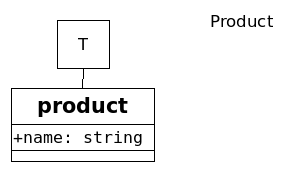
\includegraphics[scale=0.5]{dimensionProduct}
		\label{image:product}
		\caption{The product dimension.}
		\end{figure}
	\end{minipage}
	\begin{minipage}{0.45\textwidth}
	\begin{figure}[H]
	\centering
	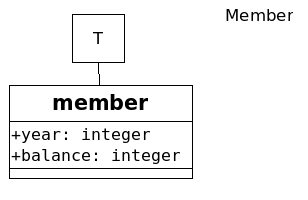
\includegraphics[scale=0.5]{dimensionMember}
	\label{image:member}
	\caption{The member dimension.}
	\end{figure}
	\end{minipage}
	
	\begin{minipage}{0.45\textwidth}
	\begin{figure}[H]
	\centering
	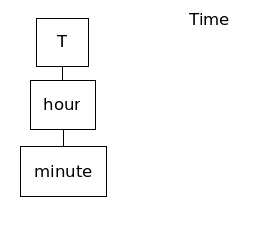
\includegraphics[scale=0.5]{dimensionTime}
	\label{image:time}
	\caption{The time dimension.}
	\end{figure}
	\end{minipage}
	\begin{minipage}{0.45\textwidth}
	\begin{figure}[H]
	\centering
	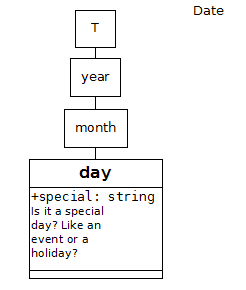
\includegraphics[scale=0.5]{dimensionDate}
	\label{image:date}
	\caption{The date dimension.}
	\end{figure}
	\end{minipage}
	
	The star schema for it can be seen below.  With the schema it is important to note that the dimensions have a surrogate key with a serial integer(it auto increments).
	
	
	\begin{figure}[H]
	\centering
	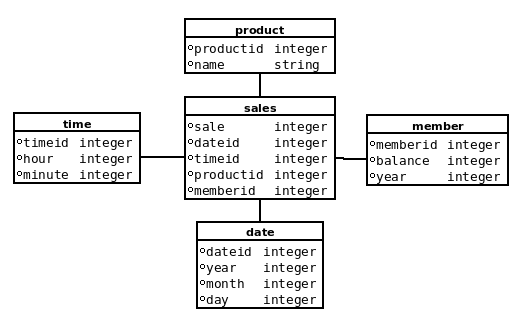
\includegraphics[scale=0.75]{star-scheme}
	\label{image:starschema}
	\caption{The star schema for the data warehouse.}
	\end{figure}
		
	

\end{document}
